	\chapter{Modèle OSI}
	\begin{figure}[H]
		\centering
		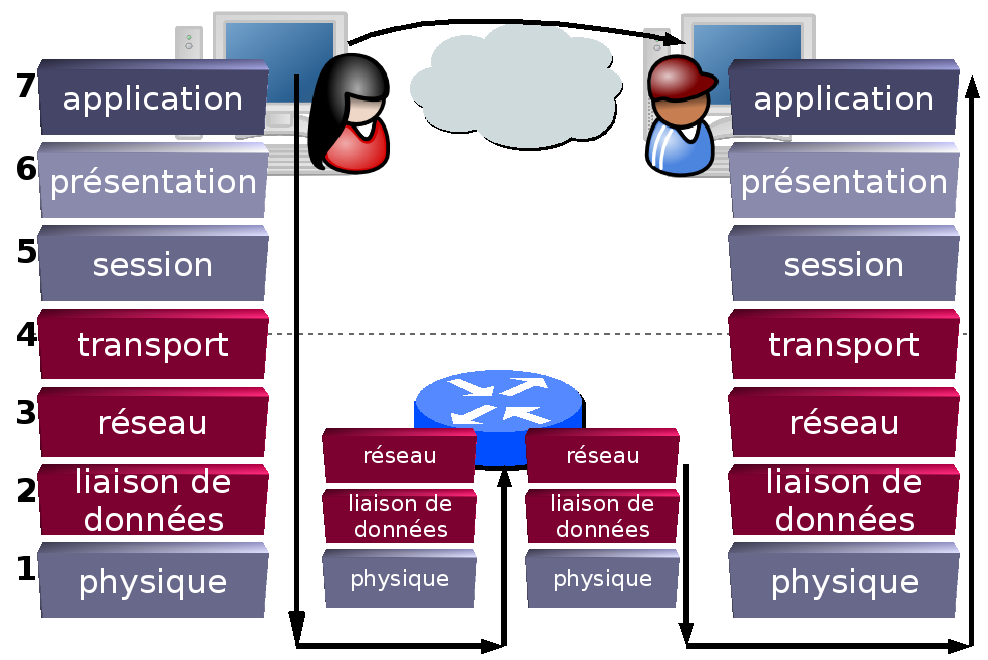
\includegraphics[width=13cm]{osi-model.png}
	\end{figure}
	\begin{description}
		\item[Application]
		\item[Présentation]
		\item[Session]
		\item[Transport] Contrôle de bout en bout
		\item[Réseau] Routage, IP, Adressage, contrôle de congestion
		\item[Liaison de données] Ethernet. Contrôle de flux, contrôle d'erreur
		\item[Physique] Transforme les données en signal
	\end{description}
	\begin{description}
		\item[Notion de service] la couche offre des services à la coche immédiatement supérieur en s'appuyant sur ceux offerts par celle immédiatement inférieure.
		\item[Notion d'encapsulation] Comment encapsuler le données venant de la couche supérieur pour --- les services offert à la couche
	\end{description}

	\chapter{Couche réseau}
	\section{Connexion}
	\begin{description}
		\item[Connexion] S'assurer de la présence du destinataire avant de communiquer
	\end{description}
	\begin{exemple}
		\begin{itemize}
			\item Le téléphone, celui-ci nécessite une connexion préalable. Les ressource sont réservées pour la communication sur les n\oe{}uds
				intermédiaires.
		\end{itemize}
	\end{exemple}
